\chapter{Resultados y discusi\'on}
\label{ch:resAuger}

\section{C\'alculo de la exposici\'on}
\label{sc:expoNu}	
	
	
	
	\subsection{Combinaci\'on de los an\'alisis}
	
	\begin{figure}[h!]
		\begin{center}
			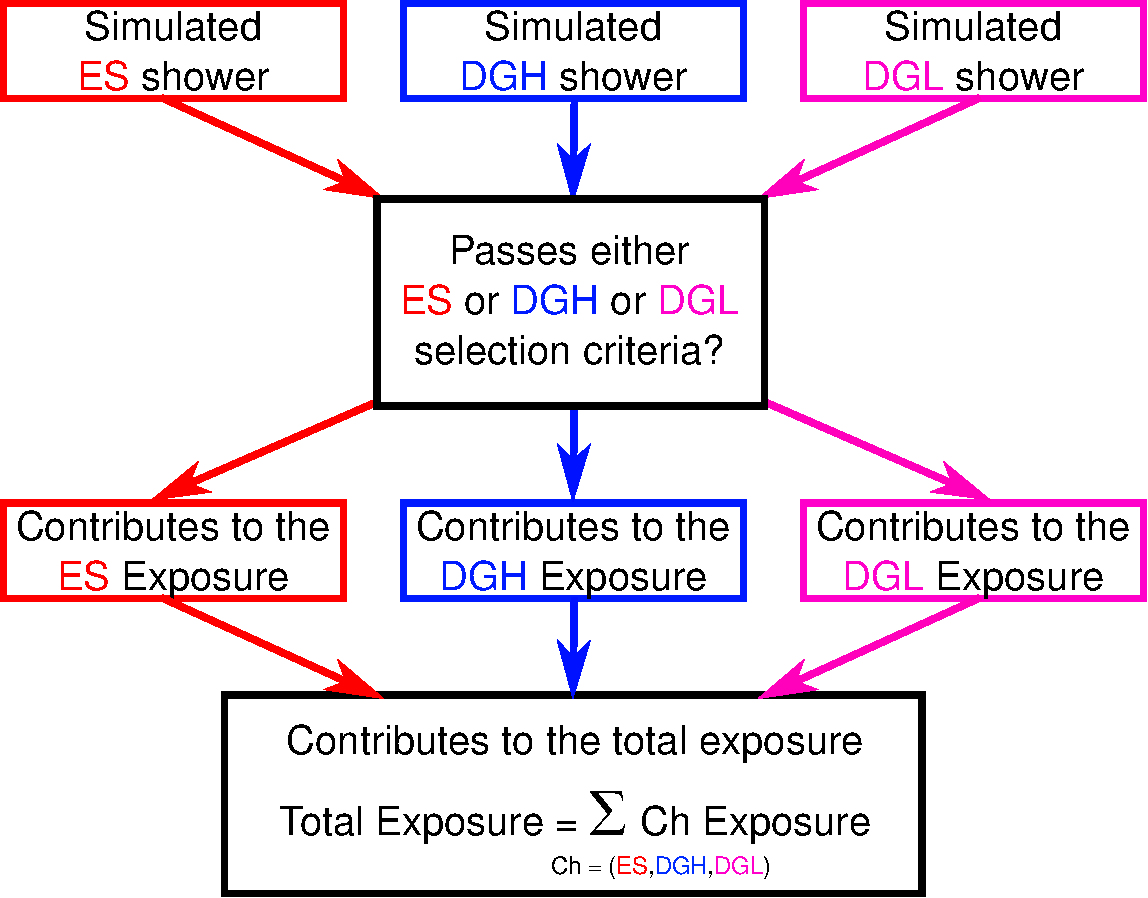
\includegraphics[width=0.9\textwidth]{fig/resultadosAuger/sketch_combined_4}
			\caption{asd}
			\label{fig:}
		\end{center}
	\end{figure}
	
% 	you are right, these numbers are important. I will work on that after the ICRC. For the moment I can only give you the exposure contribution (gain) in an E^{-2} scenario matrix, and it looks like:
% 
%           &    ES crit    &    DGH crit    &     DGL crit
% ES sh     &    0.695      &    0.035       &     neglect.
% DGH sh    &    0.045      &    0.185       &     neglect.
% DGL sh    &    neglect.   &    neglect.    &     0.04
% 
% please take into account that we have a systematic error of 40%. 
% for instance, from the table you can see that 3.5% of the total limit to an E^-2 flux is due to simulated 
% ES neutrinos selected by the DGH analysis. This gives an idea of the probability of "missclassification", but its no so simple, since the most of the ES simulated neutrinos that passes ES crit, also passes the DGH crit with a high reconstructed angle...
% In any case, if any of the three analysis finds a candidate we will have to scrutinize it with as many eyes 
% as possible and try to (1) make sure it is a neutrino and not a detector fluke, and (2) identify it as ES or 
% Down-Going quasi-horizontal, something that might not be that easy. 
	
	\begin{figure}[h!]
		\begin{center}
			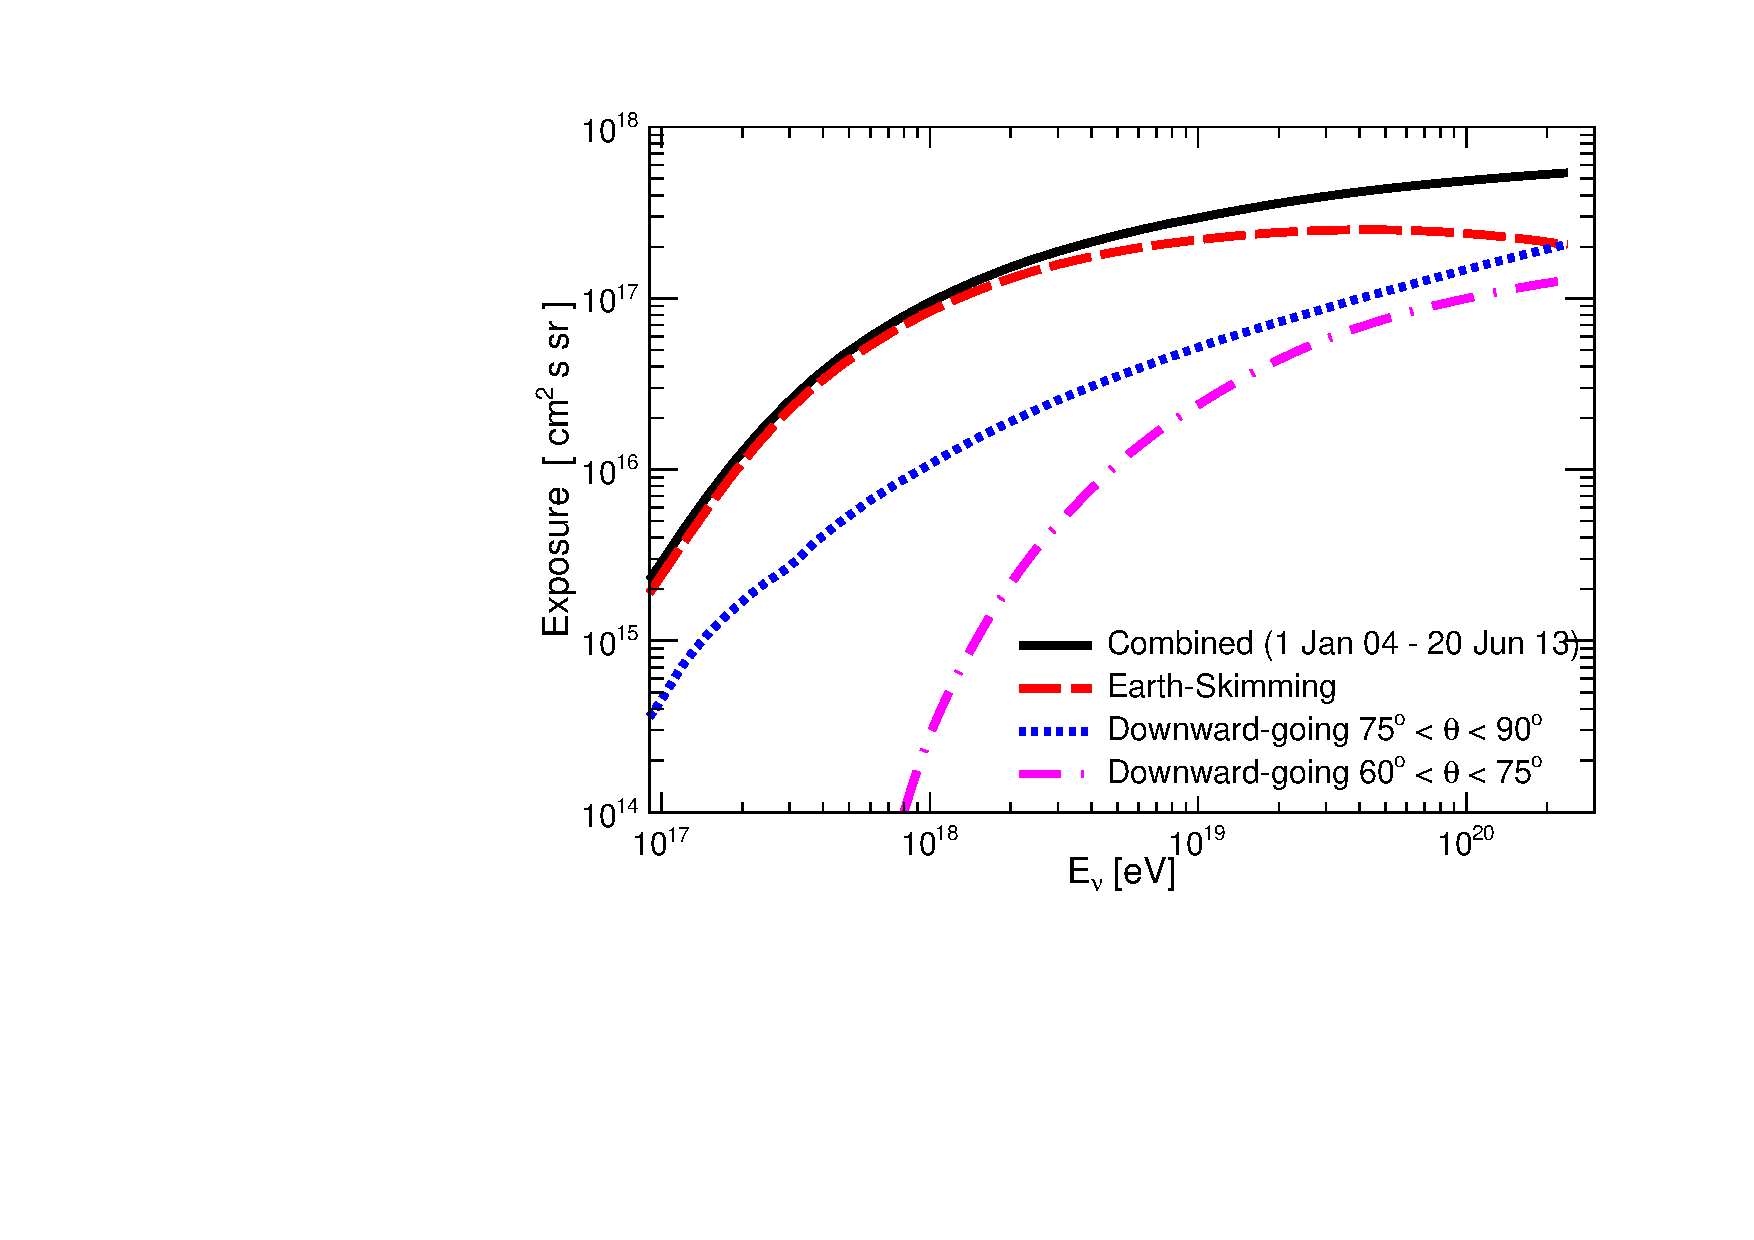
\includegraphics[width=0.9\textwidth]{fig/resultadosAuger/exposure_combined_ageing}
			\caption{asd}
			\label{fig:}
		\end{center}
	\end{figure}

	
	\subsection{Envejecimiento del detector}
	
	\begin{figure}[h!]
		\begin{center}
			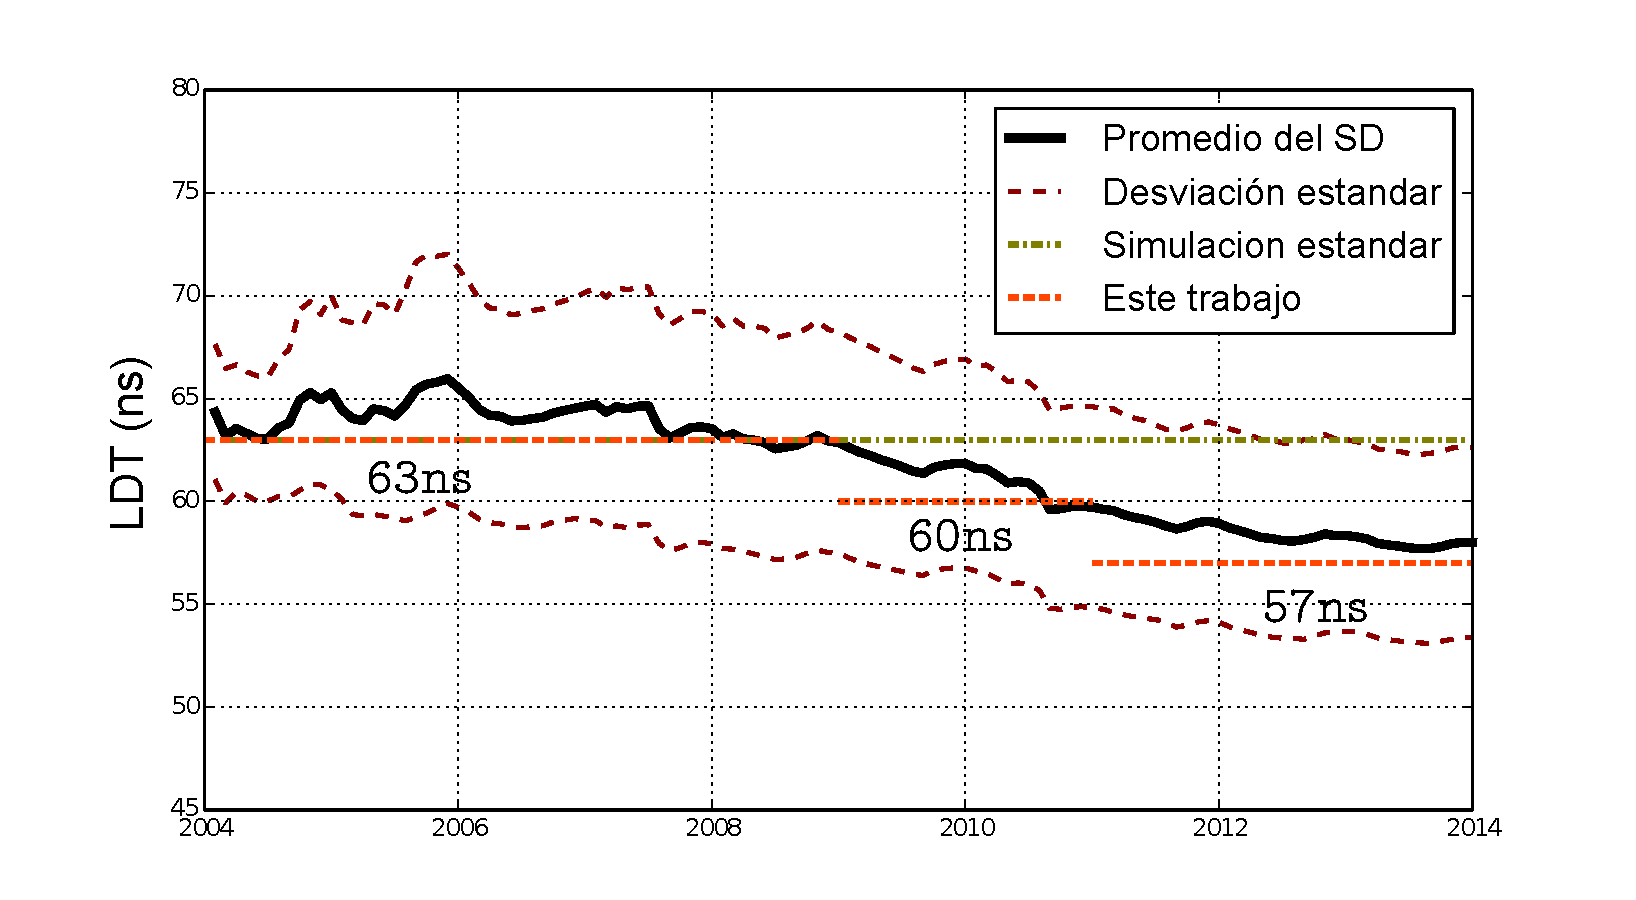
\includegraphics[width=\textwidth]{fig/resultadosAuger/timeEvolution}
			\caption{asd}
			\label{fig:}
		\end{center}
	\end{figure}
	
	\begin{figure}[h!]
		\begin{center}
			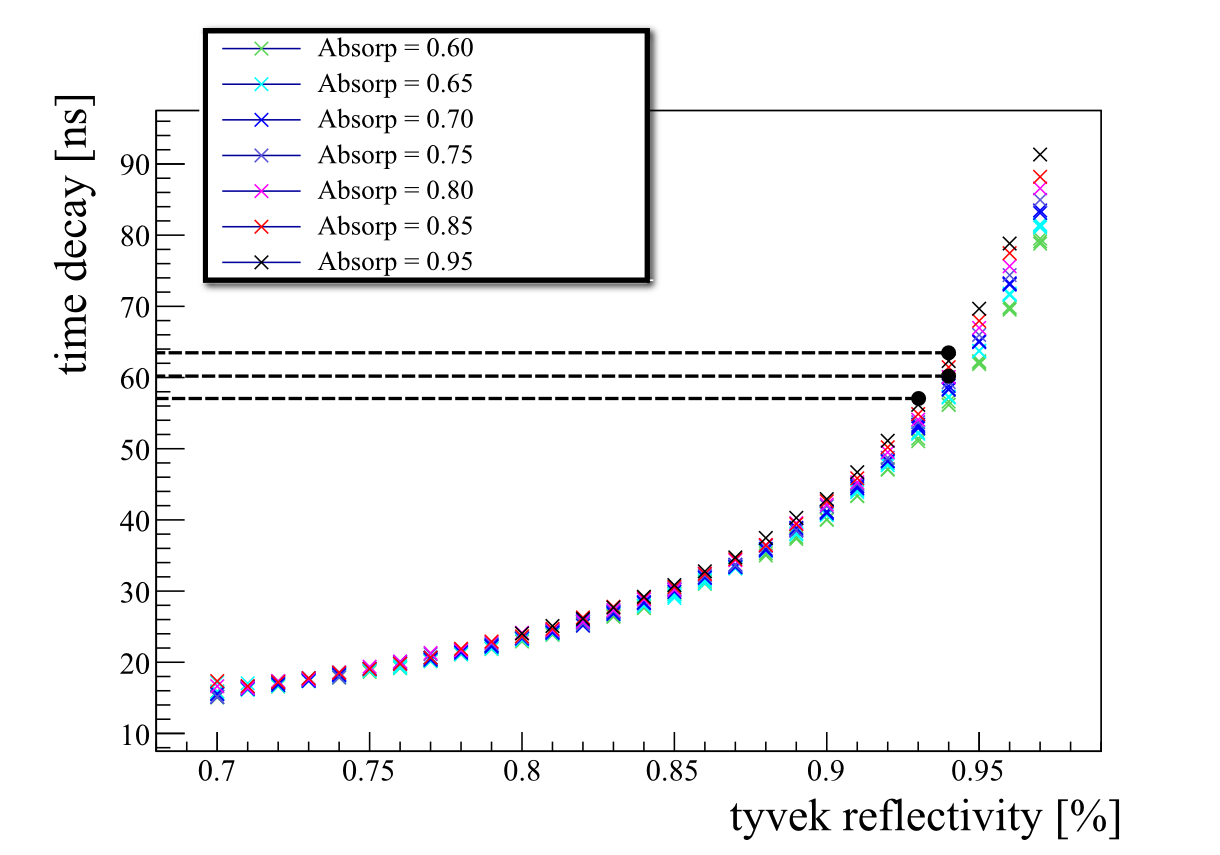
\includegraphics[width=0.9\textwidth]{fig/resultadosAuger/timedecay_vs_reflect_absorp}
			\caption{asd}
			\label{fig:}
		\end{center}
	\end{figure}
	
	\begin{figure}[h!]
		\begin{center}
			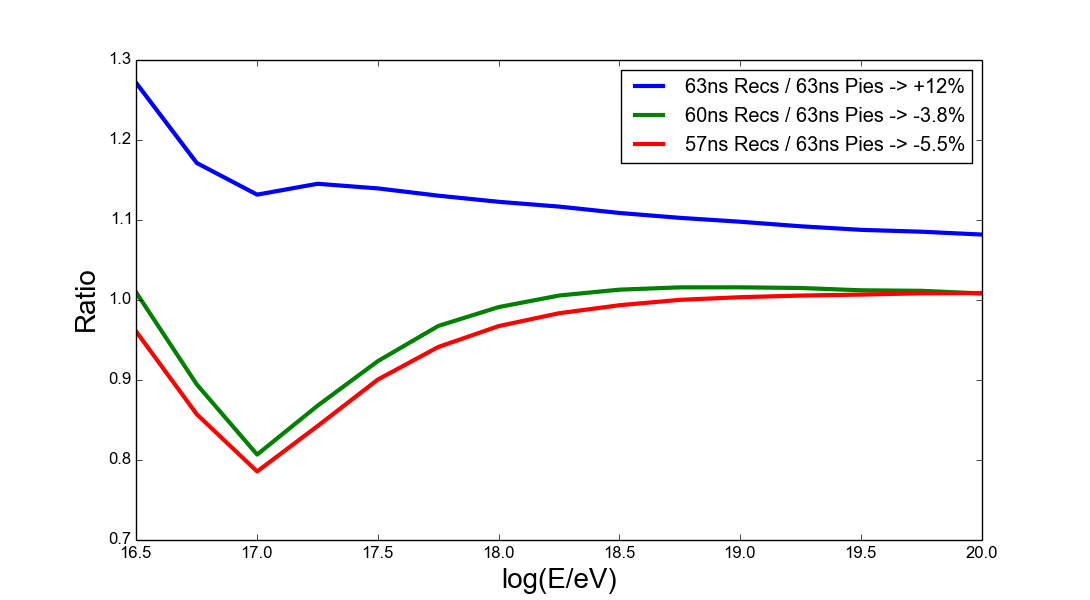
\includegraphics[width=0.9\textwidth]{fig/resultadosAuger/exposure_Arrays}
			\caption{asd}
			\label{fig:}
		\end{center}
	\end{figure}
	
	\begin{table}[h!]
	\centering
	 \begin{tabular}{l|ccc|c|c}
				Period       & tyRef & wAbs & LDT        & Exp Contrib  &   Exp Change \\
				\hline
				$[2004 - 2008]$ & 0.94  & 100  & $\sim63$ns & $33.2\%$     &   $+12\%$ \\
				$[2009 - 2010]$ & 0.94  & 80   & $\sim60$ns & $25.6\%$     &   $-3.8\%$\\
				$[2011 - 2013]$ & 0.93  & 100  & $\sim57$ns & $41.2\%$     &   $-5.5\%$\\
			\end{tabular}
	\end{table}
	
	
\section{Errores sistem\'aticos}
			
	\begin{table}[h!]
	\centering
	\footnotesize
		\begin{tabular}{|c|c|c|c|c|}
		\hline
		Source of  & ES        & DGH       & DGL        & Combined         \\
		systematic & ($90^\circ,95^\circ$) & ($75^\circ,90^\circ$) & ($65^\circ,75^\circ$) & ES / DGH / DGL   \\
		\hline
		& {\tiny \bf GAP 2013-100}     & \multirow{2}{*}{\tiny \bf PRD 84, 2011}    &   \multirow{2}{*}{\tiny \bf GAP2013-013} & \multirow{2}{*}{\tiny \bf 83.9\% / 13.7\% / 2.4\% }\\
		& {\tiny \bf PRD 79, 2009}     &     &  &  \\
		\hline
		
		Int. generator                   	    &  not eval.    &   0\%, -7\%     &   +3\%, -4\%  & +0.07\%, -1.0\% \\
		
		\hline
		
		pdf in generator                &  not eval.    &   0\%, -7\%     &   +4\%, -5\%  & +0.1\%, -1.0\% \\
		
		\hline
		
		EAS simulation	                     	    &  not eval. &   0\%, -17\%    &   +17\%, 0\%  & +0.4\%, -2.3\% \\
		
		\hline
		
		Hadronic model                  		    & +4.7\%, -1\%      &  +5\%, -2\%     &   +0\%, -6\%  & +4.6\%, -1.3\% \\
		
		\hline
		Thinning                                        & +0.3\%, 0\%   &  +7\%,  0\%     &   +7\%,  0\%  & +1.1\%, -0.0\% \\
		\hline
		Detector simulator                              & not eval.     &  not eval.      &   +5\%,  -5\% & +0.1\%, -0.1\% \\
		\hline
		\hline
		{\bf $\bm{ \sigma_{\nu_\tau}\ \otimes\ \tau}$ E-loss}    & \multirow{2}{*}{\textcolor{Red}{+40\%, -33\%}}  & \multirow{2}{*}{+9\%, -9\%}  & \multirow{2}{*}{+7\%, -7\%} & \multirow{2}{*}{\bf +33.6\%, -27.7} \\
		$\sqrt{H^2+I^2}$                                     &                 &                 &             & \\
		\hline
		\hline
% 				%%%%%%%%%%%%%%%%%%%%%%%%%%%%%%%%%%%%%%%%%%%%%%%%%%%%%%%%%%%%%%%%%%%%%%%%%%%%%%%%%%%%%%%%%%%%%%%%%%
		{\bf Topography} 	                            &  +18\%, 0\%    & included & not applicable   & +15.1\%, 0\%  \\

		\hline
		\hline
		{\bf Total}                     &  \multicolumn{3}{c|} {}  & {\bf +37.1\%, -27.9\%}         \\
		\hline
		%%%%%%%%%%%%%%%%%%%%%%%%%%%%%%%%%%%%%%%%%%%%%%%%%%%%%%%%%%%%%%%%%%%%%%%%%%%%%%%%%%%%%%%%%%%%%%%%%%
		\end{tabular}
	\end{table}

\section{Analisis ciego}

	\subsection{Abriendo la caja}
	
	\subsection{L\'imite al flujo difuso y diferencial}
	\begin{figure}[h!]
		\begin{center}
			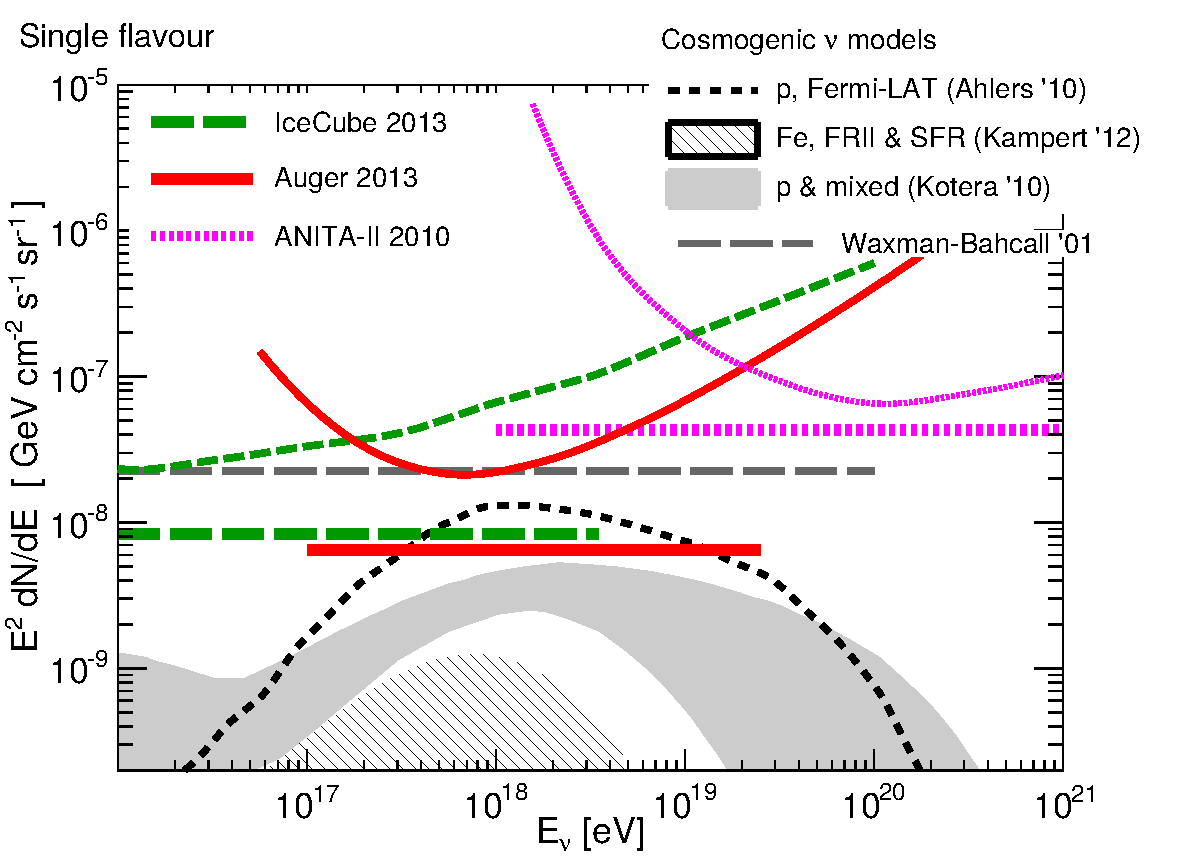
\includegraphics[width=0.9\textwidth]{fig/resultadosAuger/limits_combined_ageing}
			\caption{asd}
			\label{fig:}
		\end{center}
	\end{figure}
	
	\begin{table}[h!]
		\begin{center}
		\renewcommand{\arraystretch}{2.0}
			\begin{tabular}{|c|c|} 
			\hline
			Diffuse flux       &  Expected number of events   \\
			Neutrino Model     &  (1 Jan 04 - 20 Jun 13)   \\
			\hline
			\hline
			Cosmogenic (Kampert {\it et al.}) - proton, FRII      &  \textcolor{Red}{$\sim$ 4.0}  \\
			\hline
			Cosmogenic (Ahlers {\it et al.}) - proton, Fermi-LAT  &  \textcolor{Red}{$\sim$ 3.2}  \\
			\hline
			Cosmogenic (Kampert {\it et al.}) - proton, SFR       &  \textcolor{Blue}{$\sim$ 0.9}  \\
			\hline
			Cosmogenic (Kotera {\it et al.}) - band               &  \textcolor{Blue}{$\sim$ 0.5 $-$ 1.4}  \\
			\hline
			Cosmogenic (Kampert {\it et al.}) - iron, FRII        &  $\sim$ 0.3  \\
			\hline
			\end{tabular}
		\end{center}
	\end{table}
	

	
	\begin{figure}[h!]
		\begin{center}
			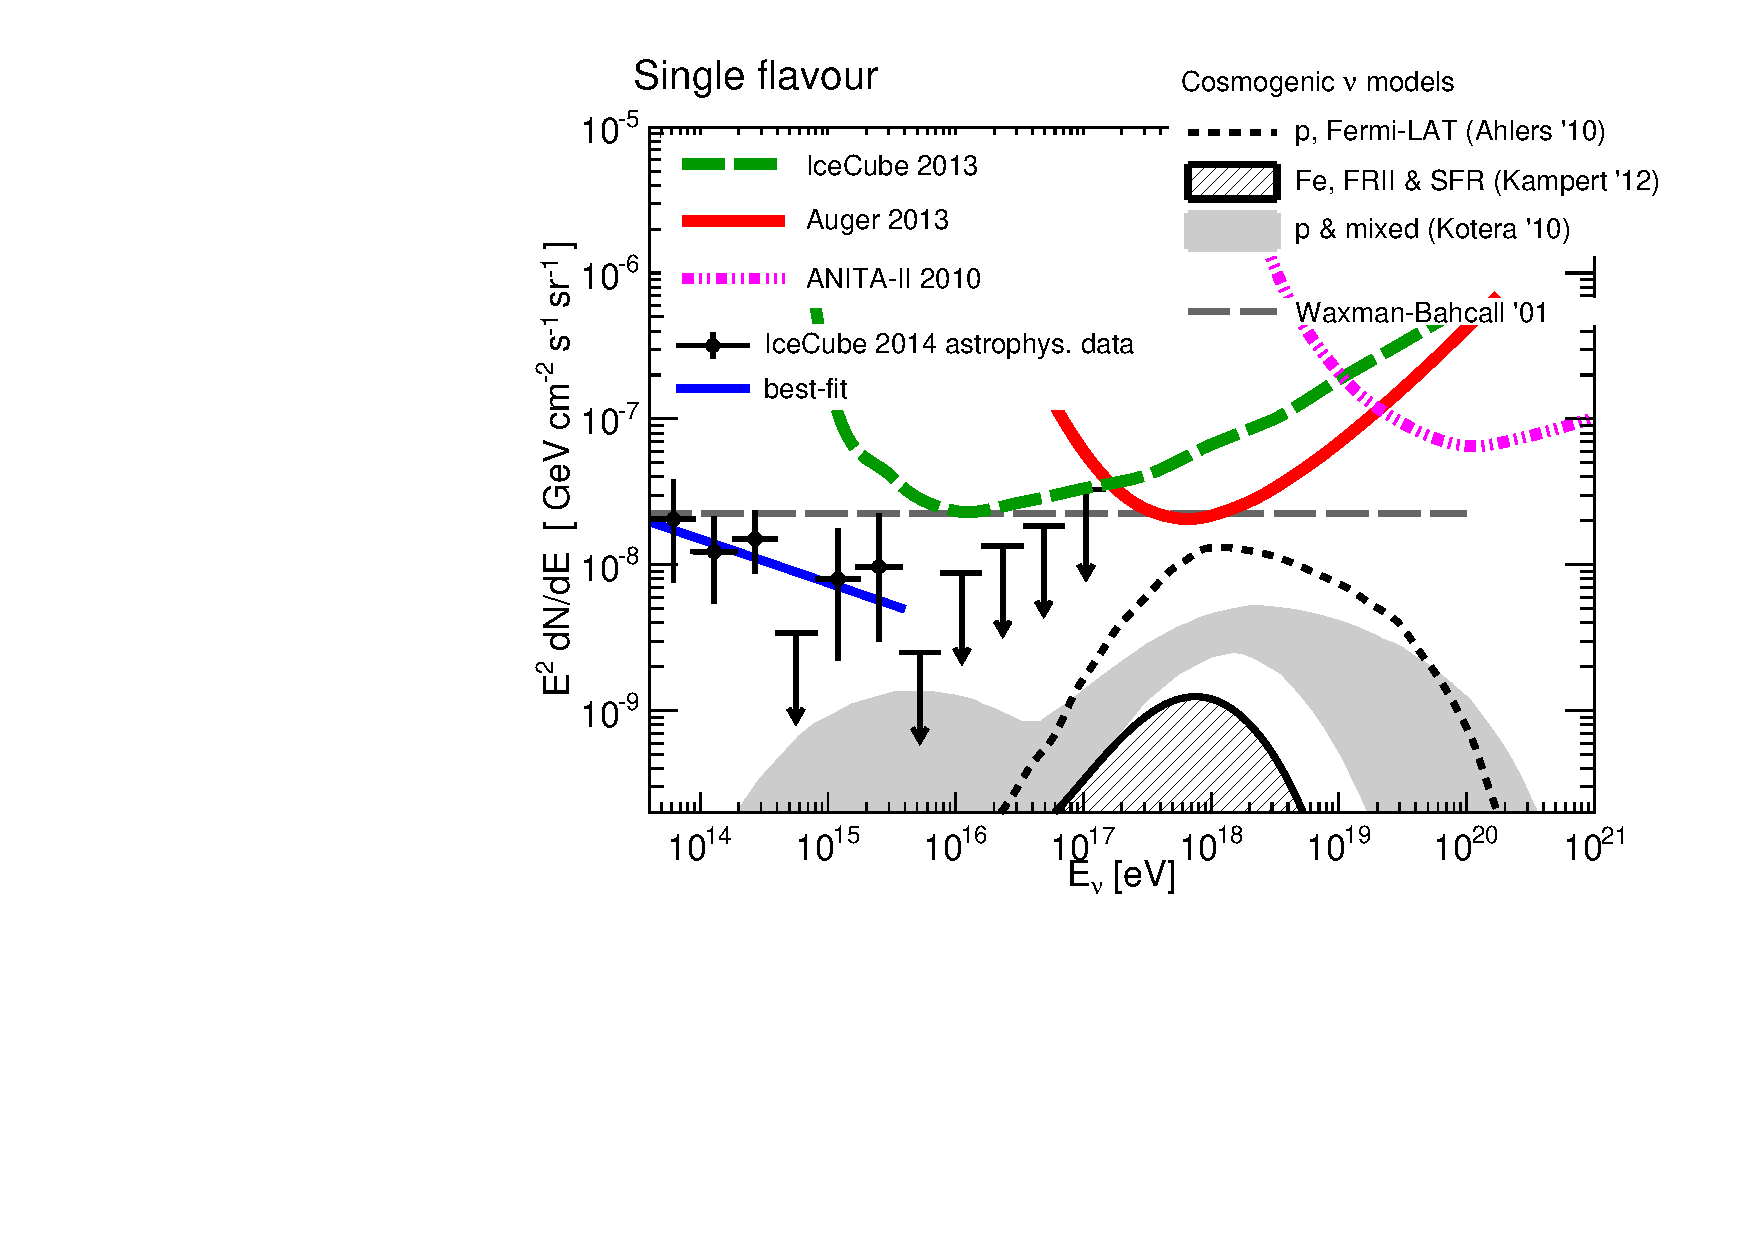
\includegraphics[width=0.9\textwidth]{fig/resultadosAuger/diff_limits_and_many_models_IceCube_data_noextrap}
			\caption{asd}
			\label{fig:}
		\end{center}
	\end{figure}

	
	